%-----------------------------------------------------------------------------
%
%               Template for sigplanconf LaTeX Class
%
% Name:         sigplanconf-template.tex
%
% Purpose:      A template for sigplanconf.cls, which is a LaTeX 2e class
%               file for SIGPLAN conference proceedings.
%
% Guide:        Refer to "Author's Guide to the ACM SIGPLAN Class,"
%               sigplanconf-guide.pdf
%
% Author:       Paul C. Anagnostopoulos
%               Windfall Software
%               978 371-2316
%               paul@windfall.com
%
% Created:      15 February 2005
%
%-----------------------------------------------------------------------------


%\documentclass[preprint]{sigplanconf}
\documentclass[11pt]{sigplanconf}

% The following \documentclass options may be useful:
%
% 10pt          To set in 10-point type instead of 9-point.
% 11pt          To set in 11-point type instead of 9-point.
% authoryear    To obtain author/year citation style instead of numeric.

\usepackage{yfonts}
\usepackage{amsmath}
\usepackage{amsthm}
\usepackage{amssymb}
%\usepackage{mathpartir}
\usepackage[colorlinks=true,
citecolor=citec,
linkcolor=linkc,
urlcolor=urlc,
]{hyperref}
\usepackage{url}
\usepackage{graphics}
\usepackage{graphicx}
\usepackage{wasysym}
\usepackage{harmony}
\usepackage{marvosym}
\usepackage{multirow}
\usepackage{xspace}
\usepackage[nameinlink,nosort]{cleveref}
\usepackage{xeCJK}
\usepackage[usenames,dvipsnames]{xcolor}
\usepackage[utopia]{mathdesign}
\usepackage{natbib}
\usepackage{ulem}
\usepackage[mathcal]{euscript}
\usepackage[linesnumbered,ruled]{algorithm2e}

\renewcommand{\UrlBreaks}{\do\/\do\a\do\b\do\c\do\d\do\e\do\f\do\g\do\h\do\i\do\j\do\k\do\l\do\m\do\n\do\o\do\p\do\q\do\r\do\s\do\t\do\u\do\v\do\w\do\x\do\y\do\z}


% ____________________________________________________________
% Listings Package Configuration
% \usepackage[scaled]{beramono}

%\renewcommand*\ttdefault{txtt}
\usepackage[T1]{fontenc}
% \usepackage{inconsolata}

\definecolor{citec}{RGB}{128,0,64}
\definecolor{linkc}{RGB}{0,64,128}
\definecolor{urlc} {RGB}{128,64,0}

\setCJKmainfont{HeiseiMinStd-W5}[Path = ./]
\setmonofont{Inconsolata-Regular}[Path = ./]

\newfontfamily\birbaslo{BirbasloText}[Path = ./]

% This Deep Tex Voodoo is from
%   <http://www.latex-community.org/forum/viewtopic.php?f=5&t=2072>
% It's purpose is to make \lstinline normal size, without affecting
% \lstinputlisting.  It seems to work but I have no idea how or why,
% and I rather hope never to learn.
%\makeatletter
%\lst@AddToHook{TextStyle}{\let\lst@basicstyle\ttfamily\normalsize}
%\makeatother

\begin{document}

\conferenceinfo{{\birbaslo sigbovik~'20}}{pittsburgh, PA, USA}
\copyrightyear{2020}
\copyrightdata{}

\title{
% how to \texttt{git bisect} when your test suite hates you
% how to \texttt{git bisect} when your test suite is a hater
how to \texttt{git bisect} when your test suite is having a bad day
% how to {\tt git bisect} when yr test suite is just, trying its best ok % there we go
}
% \subtitle{\em The Randomly-Scoped Lambda Calculus}
% \subtitle{Subtitle Text, if any}
% \subtitle{a probability puzzle}

\authorinfo{ben blum}{}{bblum@alumni.cmu.edu}

\maketitle

\begin{abstract}
	I like probability puzzles but don't know enough stats to actually solve them properly
	so I threw some thinking sand at it and learned some interesting stuff anyway.
\end{abstract}

% \category{D.D.R.}{Exercise and Fitness}{Arcade Dance Games}

\keywords pdflatex
% bracket, groove, in, jumps, the

\newcommand\confidents{\ensuremath{\mathcal{Z}}\xspace}
\newcommand\pdf{\ensuremath{\mathsf{pdf}}\xspace}
\newcommand\cdf{\ensuremath{\mathsf{cdf}}\xspace}

\section{problem statement}

Let's say you're trying to bisect
% a bug in
a given range of $n$ commits.%
\footnote{To use binary search to find a commit that introduced a bug.}
Call them $c_0 \dots c_{n-1}$, where $c_0$ is known safe and $c_n$ is known to have the bug.
You'd probably start by testing $c_{n/2}$, right?
And you'd expect to pinpoint the buggy comit in $\mathsf{log} (n)$ steps.
That's math.

Ok, but what if the bug reprodues nondeterministically with some probability $p<1$.
You can't even pinpoint the bug at some $c_{b}$ for sure anymore;
you can at best know
that it \textasciitilde{}prooobably\textasciitilde~won't reproduce in any $c_{i<b}$,
with some confidence $\confidents$.
Now evaluate your strategy by the expected number of steps to achieve, let's say for tradition's sake, $\confidents \ge 0.99999$.
Is it still optimal to bisect at the midpoint?%
\footnote{Spoiler: No, or I wouldn't have bothered with this paper.}
What would be a better strategy, as a function of $p$?

%%%%%%%%%%%%%%%%%%%%%%%%%%%%%%%%%%%%%%%%%%%%%%%%%%%%%%%%%%%%%%%%%%%%%%%%%%%%%%%%

\section{intermission}

Put the paper on pause now and think about it.
No, really, give it a go!
I mean, if you don't think math puzzles like this are cool, just stop reading, no worries.
I'm sure there's a paper about, like, hygienic image macros or empire machines or something for you just a few page-turns away.
% I'm sure tom7 is up to some wacky hijinks or something just a few page-turns away.

If you're feeling adventurous,
implement a strategy and throw it in this simulator I implemented to see how it stacks up:
\url{https://github.com/bblum/sigbovik/blob/master/bisect}.
You just gotta implement {\tt trait BisectStrategy},
and it even does all the hard work of applying Bayes's rule
%computing the
%distribution of
%priors with Bayes's rule
for you and letting you see the PDF and everything.
Check it out.


%%%%%%%%%%%%%%%%%%%%%%%%%%%%%%%%%%%%%%%%%%%%%%%%%%%%%%%%%%%%%%%%%%%%%%%%%%%%%%%%

\section{pdfs, but not the portable document format kind, and our friend rev. bayes}

Ok, so let's model the problem as a sequence of steps on a probability distribution function
(henceforth, PDF; and also, CDF for the cumulative kind).
Initially, $\pdf(i) = 1/n$ for all $0 \le i < n$.
When the bug reproduces at some commit $b$,
you're certain no $c_{i>b}$ introduced the bug, so each $\pdf(i>b)$ becomes $0$,
and each $\pdf(i\le b)$ renormalizes by a factor of $n/b$, to preserve the $\int \pdf(i) \text{d} i = 1$ invariant.%
\footnote{Implemented as {\tt fn adjust\_pdf\_bug\_repros()} in the simulator.}

In the deterministic case ($p=1$),
the symmetric thing happens when the test passes at some $c_j$: $\pdf(i\le j) = 0$.
But when $p<1$, we must generalized it \cite{mario3}. Here's Bayes's rule:
\[
P(A|B) = \frac{P(B|A) \times P(A)}{P(B)}
\]

\newcommand\renorm[1]{\ensuremath{\mathcal{R}_{#1}}\xspace}

In this case, $B$ is that the test passes at $c_j$, and $A$ is that bug exists at or before $c_j$ after all.
$P(B|A)$ is the false negative rate, i.e. $1-p$.
$P(A)$ is the prior on $c_j$ containing the bug, i.e., $\cdf(j)$.
And $P(B)$ is the false negative rate weighted by the bug existing, i.e., $(1-p)\cdf(j) + 1(1-\cdf(j))$.
% simplifies to: cdf(j) - p*cdf(j) + 1 - cdf(j)
% simplifies to: 1 - p*cdf(j)
To update our priors on commits up to $j$, we renormalize by dividing out the old $\cdf(j)$
and multiplying by the new $P(A|B)$, i.e.,
%To update our priors on commits up to $j$, we divide out the old $\cdf(j)$
%and multiply by the new $P(A|B)$.
%Call this renormalization factor $\renorm{j}{i}$.
%\[
%	\forall i \le j \Rightarrow \renorm{i}{i} = 
%	\frac{1}{\cdf(j)}
%	\frac{(1-p)\cdf(j)}{(1-p)\cdf(j) + (1-\cdf(j))}
%\]
\[
	\forall i \le j, \pdf'(i)
	\leftarrow
	\pdf(i)
	\frac{1}{\cdf(j)}
	\frac{(1-p)\cdf(j)}{(1-p)\cdf(j) + (1-\cdf(j))}
\]
Which simplifies to:
\[
	\forall i \le j, \pdf'(i)
	\leftarrow
	\pdf(i)
	\frac{1-p}{1 - p\cdf(j)}
\]
Call this renormalization factor $\renorm{}$.
As a sanity check, $p\cdf(j)$ is less than $p$, so $\renorm{i\le j} < 1$.

Likewise, for commits above $j$, we have $P(B|A) = 1$, $P(A) = 1-\cdf(j)$, and $P(B)$ the same as before.
Renormalizing from $1-\cdf(j)$ this time (and skipping the unsimplified version), we get:
\[
	\forall i > j, \pdf'(i)
	\leftarrow
	\pdf(i)
	\frac{1}{1 - p\cdf(j)}
\]
As a sanity check, $p\cdf(j)$ is positive, so $\renorm{i > j} > 1$.
If you like pen-and-paper algebra, you can also see that
$
\cdf(j)
\renorm{i \le j}
+
(1-\cdf(j))
\renorm{i>j}
= 1$.%
\footnote{Implemented as {\tt fn adjust\_pdf\_no\_repro()} in the simulator.}


Let's do a nice concrete example.
Say $n=16$, the test passes at $j=7$, and then the bug repros at $j=11$.
In the deterministic case, all the probability mass will be concentrated uniformly in the range $[8,11]$.
However, if the bug repros only half the time,
%the renormalization factors around $c_7$ come out to $2/3$ and $1/3$
$\renorm{i \le 7} = 2/3$
and
$\renorm{i > 7} = 4/3$,
and we get probability mass scattered all the way down to $c_0$,
as shown in \Cref{fig:example}(a).
Yuck, someone clean that up!

Now let's say the test passes at $j=9$, then at $j=10$.
\Cref{fig:example}(b) shows the updated PDFs/CDFs:
for $p=1$, this pinpoints the bug at $j=11$, and the search is over.
But for $p=0.5$, there's still 2/3 odds we'd be wrong!
In fact, from here it takes 18 further probes at $j=10$ until we are at least five 9's confident that $c_{11}$ is the culprit.%
\footnote{See {\tt fn test\_figure\_1()}!}
Bayes's rule gonna get ya.

% cdf 9 -- 0.75
% 
% R- = 1/2 / 1-((3/4)/2)
% R- = 1/2 / 5/8
% R- = 8/10 = 4/5
% 
% R+ = 1 / 5/8
% R+ = 8/5 = 16/10

% cdf 10 - 0.8
% 
% R- = 1/2 / 1-((4/5)/2)
% R- = 1/2 / 6/10
% R- = 10/12 = 5/6
% 
% R+ = 1 / 6/10
% R+ = 10/6

\begin{figure}[t]
	\begin{tabular}{c}
	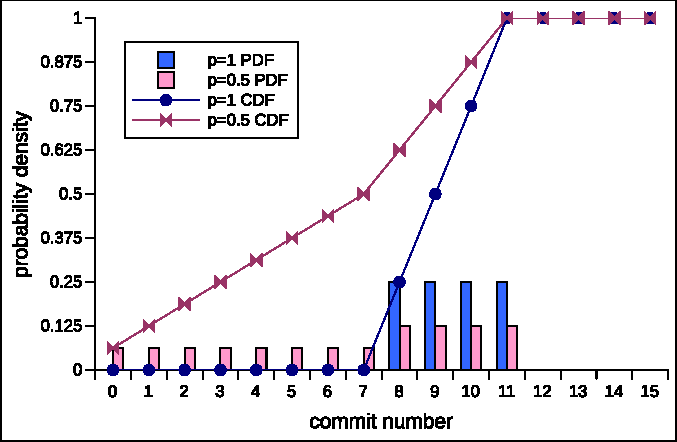
\includegraphics[width=0.45\textwidth]{example.pdf}
	\\
		(a) After two tests.
		\\
		\\

	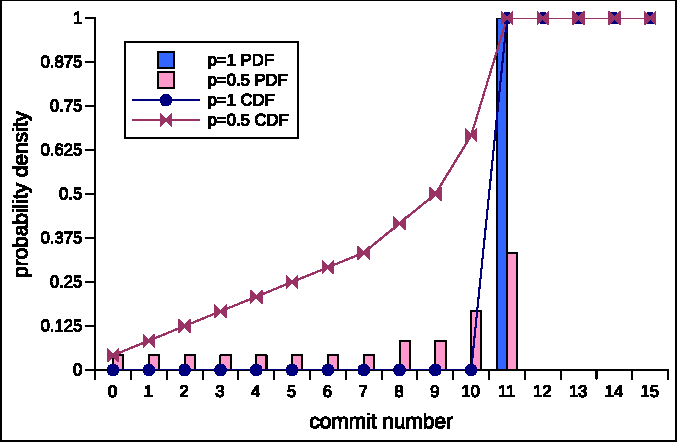
\includegraphics[width=0.45\textwidth]{example2.pdf}
	\\
		(b) After ``classical`` search terminates.
	\end{tabular}
	%\caption{Example deterministic and nondeterministic PDFs and CDFs.}
	\caption{Example \{,non\}deterministic \{P,C\}DFs.}
	\label{fig:example}
\end{figure}

A noteworthy invariant here is that the PDF is always monotonically nondecreasing in its nonzero range:
each passing test always shifts probability mass to the right of the bisect point,
but past the earliest known bug repro, nothing can ever revive it back above 0.

%%%%%%%%%%%%%%%%%%%%%%%%%%%%%%%%%%%%%%%%%%%%%%%%%%%%%%%%%%%%%%%%%%%%%%%%%%%%%%%%

\section{prior work}

I was kinda surprised to find no existing mathy solution to this problem lying around on the online.
Wikipedia has a brief little subsection on ``noisy binary search'', which links a few papers older than I am.
In one \cite{noisy2}, they bound the number of erroneous answers by a fixed factor of the number of queries,
so it's more like ``twenty questions with lies'' than bisect.
In another \cite{noisy1}, they do fix the error rate $p$,
but they allow for symmetric false negatives and false positives, both with the same $p$.
This too changes the nature of the problem;
notably, if $p=0.5$, you can't make any progress whatsoever.

Dropbox has a CI service called Athena \cite{athena}
which automatically searches for flaky tests, when otherwise no bug exists.
In this case the goal is to keep the build green, but if you consider the flaky test itself to be the bug, it's the same problem.%
\footnote{Incidentally, the symmetric case
-- where a bug repros with $p=1$, but the test also flakes with some $q<1$ --
is also the same problem.}
Athena's ``deflakes'' the test at each commit by running 10 times,
treating the combined result as ``basically as good as $p=1$'',
and then runs an otherwise classical binary search.%
\footnote{Upcoming, I will call this strategy \textsf{Human-Mistrustful}$(10)$.}
In this setting, $p$ is not known in advance, so using Bayes's rule is off the table.
But I will show that even without access to the PDF, a better strategy exists. % at least by my definition

%%%%%%%%%%%%%%%%%%%%%%%%%%%%%%%%%%%%%%%%%%%%%%%%%%%%%%%%%%%%%%%%%%%%%%%%%%%%%%%%

\section{strategies}

Ok, so how do we
%cope with the fact that we'll never have a proper lower bound?
%How do we
make progress,
i.e., concentrate probability mass til there's $\confidents$ of it in one place,
as quickly as possible?
%In principle, testing anywhere in the range $[0,b)$,
%where $b$ is the earliest known buggy commit,
%will make progress,
%
%% ghhh this sentence only feels good if i know what i'm talking about
Let's deconstruct the motives of classical binary search.
Let $c_b$ be the earliest known buggy commit, and $c_a$ be the latest known safe commit.
In Determinism World, bisecting at $c_{(a+b)/2}$
minimizes the worst case maximum range remaining,
as the two possible outcome ranges are the same length.
%But in Nondeterminism World,
%the worst case is a big constant times linear:
%an adversarial RNG god could pass your test a thousand times on $c_{n-1}$, then fail,
%then pass it a thousand times on $c_{n-2}$, then fail, and so on,
%before ultimately arriving at buggy commit $c_0$.
%So thinking about the worst case is not productive for a sublinear strategy,
%and also,
%we shouldn't be thinking about the range length,
%because a pass is still progress even though $a$ doesn't ever budge,
But in Nondeterminism World, $a$ doesn't ever budge from $0$,
so bisecting at $c_{(0+b)/2}$ will not even terminate.
%will eventually fail to make progress.
Sure, hitting the PDF with
%Bayes's rule at $b/2$
$\renorm{b/2}$
will always move {\it some} mass rightward,
but once five 9's of it is already over there,
%to the right of that point,
it can't concentrate it onto one point.
So let's not think about the range.

\subsection{bisect probability mass}

Another way to think about Determinism World is that the $c_{(a+b)/2}$ bisect point
% maximizes the expected probability mass that moves from one side to the other.
cuts the probability mass, rather than the range, in half,
% How about in Nondeterminism World,
% we ignore the range length, and instead bisect at the midpoint of probability mass,
i.e., $\mathsf{max}_j (i)$ s.t. $\cdf(j) \le 0.5)$.
This approach
fits the ``binary search'' spirit,
and will terminate in Nondeterminism World,
i.e.,
if $b$ is the solution, it converges to repeatedly probing $b-1$,
so it can pass any fixed $\confidents$ threshold.
%(which is more than you can say for the range-based $c_{(0+b)/2}$).
%It is intuitively obvious that this will make progress faster than bisecting at $c_{(b+0)/2}$,
%But is it fast?
% However, it doesn't maximize either the minimum or the expected amount of mass that moves:
% when $p<1$, it's intuitively apparent that this CDF threshold should actually be less than $0.5$.%
%\footnote{I did some pen-and-paper algebra to find a closed form for this,
%but I actually trust the simulator more than myself at this point,
%so I stopped spending brains on this part of the problem. I kind of regret that.}
%
%Is maximizing the expected moved mass as a function of $p$ the fastest we can go,
%and if so, why?
But is $0.5$ still the best bisect point even when $p<1$?
I wondered if this could be expressed as the amount of probability mass moved from one side to the other,
i.e., $\sum_i \mathsf{abs}(\pdf(i) - \pdf'(i))$.
In the case where the bug repros this is:
\[
	p\cdf(j) \times (1-\cdf(j))
\]
and in the case where the test passes:
\[
	(1-p\cdf(j)) \times \cdf(j) \times (1-\renorm{i\le j})
\]
which, surprisingly, simplifies to exactly the same thing as the bug repros case.
The maximum occurs where $\partial/\partial \cdf(j)$ is 0,
which turns out to be at $\cdf(j)=0.5$ after all, and independent of $p$.%
\footnote{I also worked out the {\it minimum} moved mass between the pass and fail case,
which is almost always the pass case,
and comes out to
%$\frac{p\cdf(j)(1-\cdf(j))}{1-p\cdf()}$
$\frac{\cdf(j)(1-\cdf(j))}{1/p-\cdf(j)}$,
which experiences its maximum at
$\frac{1-\sqrt{1-p}}{p}$ (thanks wolframalpha).
But this is worst-case thinking, which doesn't seem appropriate.
Let's have some optimism!}
But it's not clear that the amount of mass moved
necessarily corresponds to reaching $\confidents$ the fastest.
%It just sounds kinda nice?
%What is the best threshold, perhaps as a function of $p$, and why?


%expected moved entropy
%	call cdfj 'z' for the threshold we're looking for
%
%moved entropy at j in pass case
%	new area is z (1-p)/(1-pz)
%	old area is z
%	so:
%	z - z R
%	z (1-R)
%
%	z [ 1-pz - (1-p) ] / (1-pz)
%	z [ p-pz ] / (1-pz)
% moved entropy to the right of j, should be equal
% 	new area is (1-z)R
% 		is (1-z)/(1-pz)
% 	old area is 1-z
% 	moved area is (1-z)(R-1)
% 		is (1-z)(pz)/(1-pz)
% 		is (pz-pzz)/(1-pz) yup, checks out
% 
%
%probability that it moves = p test passes
%	1(1-z) + (1-p)z (that's B)
%	= 1-z + z-pz
%	= 1-pz (still B)
%
%so this term:
%	(1-pz) (z) (p-pz) / (1-pz)
%	= z(p-pz)
%	= pz-pzz
%
%moved entropy at j in fail case
%	new area is 1
%	old area is z
%	of course, all 1-z of that shit moves
%
%probability that it moves = p test fails
%	pz
%
%so this term:
%	pz(1-z)
%	= pz-pzz
%	(wow, that's the same?)
%
%total expected moved: 2pz-2pzz
%
%solve for derivative dz = 0 to find argmax z
%	p - 2pz = 0


\subsection{bisect entropy}

\newcommand\entropy{\ensuremath{\mathcal{H}}\xspace}

A PDF's information content is measured in entropy:
$\entropy = \sum_i \pdf(i)\mathsf{ln}(\pdf(i))$.
Alone, this value is fairly meaningless, but to compare them,
a spikier PDF has lower entropy than a flatter one.
Indeed,
when the search terminates in Determinism World, $\entropy = 0$.
I thought for a while about how to link ``minimum expected entropy''
to the stated goal %in Nondeterminism World:
of
%minimizing the expected steps until
$\confidents = \mathsf{max}_i (\pdf(i)) \ge 0.99999$,
but couldn't really formalize the idea.
The goal of five 9's is fairly arbitrary anyway,
and also not necessarily stable under the entropy measurement,
since it doesn't care how the remaining $0.00001$ is distributed.%
\footnote{See {\tt fn test\_entropy\_stability()}.}

This strategy is expensive to compute.
Whereas bisecting at some fixed threshold of probability mass merely requires a $O(\mathsf{log}  n)$ query of the CDF,
computing the expected entropy is $O(n)$ for {\it each} bisect point.
A Very Smart Math Friend of mine \cite{primer} analyzed the easy case of the initial test,
when the PDF is still uniform (i.e., $\forall i, \cdf(i) = i$),
and found the closed form
\[
	\entropy_{j,0} = p \mathsf{ln}(j)
	+
	(1-pj) \mathsf{ln} (1-pj)
	-
	j(1-p) \mathsf{ln} (j-p)
\]
whose derivative,
in his words,
``looks like a giant mess that does not admit an analytic solution for $j$.''

% even the easy case of the inn
% %the expected resulting
% $\mathsf{EV}(\entropy(\renorm{} \circ \pdf))$
% %\[
% %(\cdf(j) + (1-\cdf(j))(1-p))\entropy(\renorm \circ \pdf)
% %+
% %p(1-\cdf(j))\entropy(\renorm{\text{bug}} \circ \pdf)
% %\]
% or whatever (bleh, my notation is kinda reaching its limits here).
% %so how would you write a proof about it anyway.
% Nevertheless, it seems promising, and easy to implement.

There is a ray of hope, however:
thanks to the nondecreasing-PDF invariant I mentioned on the previous page,
the expected entropy has a unique local minimum.%
\footnote{See {\tt fn test\_expected\_entropy\_has\_unique\_local\_minimum()}.}
Thus we can binary search for the global minimum, making this at least $O(n\mathsf{log}n)$
instead of $O(n^2)$.

\subsection{bisect randomly}

Maybe a random world calls for a random algorithm!
It's obvious this will terminate, but of course it won't be fast.
Intuitively, if we use the PDF to weight the random choice, it will be faster than choosing uniformly in $[0,b)$.
But how much faster?

You can tell at this point I'm starting to get statistics fatigue.

\subsection{human}

Humans are known to be less patient than computers (citation: see previous sentence).
If a human is unwilling to compute $\renorm{} \circ \pdf$ by hand every step,
or, more prohibitively,
simply doesn't know $p$ in advance so can't compute $\renorm{}$ at all,
what should they do?

Think back to Athena from the prior work section.
The human


% parameterize over 10
% what should the human do when they think they're done? -> probe repeatedly at b-1
% what should they do when 

Regardless, it's easy to 


%%%%%%%%%%%%%%%%%%%%%%%%%%%%%%%%%%%%%%%%%%%%%%%%%%%%%%%%%%%%%%%%%%%%%%%%%%%%%%%%

\section{simulating it}

At this point I threw in the towel on the maths front,
and wrote a bunch of code to let the law of large numbers do my work for me.

To save you some page-turning, here's the source code link again:
\url{https://github.com/bblum/sigbovik/blob/master/bisect}.
A {\tt BisectStrategy}
implements a function over $p$, the PDF, and/or its own internal state
to choose the next bisect point.
The {\tt SimulationState} is initialized with fixed $n$ and $p$,
and repeatedly invokes a given {\tt BisectStrategy},
hitting the PDF with Bayes's rule accordingly,
until $\confidents \ge 0.99999$.
I provide implementations for all the strategies from the previous section.
It's written in Rust so it's self-documenting.

I learned a lot about floating point.
I don't mean like NaNs and mantissa bits,
I mean that when your problem is fundamentally a long multiplication sequence of increasingly high rationals,
your precious $\cdf(n)$ inevitably drifts ever farther from 1, and you start drowning in imprecision \cite{drowningpoint}.
I suppose I could have used the {\tt BigRational} library,
but I chose Rust over Haskell for this so I could {\it avoid} runaway memory consumption,
so I resigned myself to explicitly renormalizing my PDFs by $1/\cdf(n)$ each time I updated them.
After that, I was able to write some assertions
to bound the imprecision drift within $k(\text{\tt std::f64::EPSILON})$ \cite{epsilon}.
But yeah, I definitely spent some sanity points writing a function named {\tt fn assert\_kinda\_equals\_one(\&self)}.


%%%%%%%%%%%%%%%%%%%%%%%%%%%%%%%%%%%%%%%%%%%%%%%%%%%%%%%%%%%%%%%%%%%%%%%%%%%%%%%%

\section{evaluation}



%%%%%%%%%%%%%%%%%%%%%%%%%%%%%%%%%%%%%%%%%%%%%%%%%%%%%%%%%%%%%%%%%%%%%%%%%%%%%%%%

\section{future work}

I'm not ashamed to admit I left a lot of loose ends in this paper.
The biggest open questions for me are:
\begin{enumerate}
	\item What relates $p$ to {\sf cdfbisect}'s optimal argument?
	\item Why is {\sf entropy} {\it so tantalizingly close} to {\sf cdfbisect}? Is there some way to show they're the same?
\end{enumerate}
I have also prepared a set of backup questions in case those aren't enough for you:
\begin{enumerate}
	\setcounter{enumi}{3}
	\item If you don't know $p$ in advance, is there an efficient way to multiplex the search with figuring it out on the fly?
	\item What if false positives are also possible, with some $q \ne p$?
	\item How do you account for the cost of {\tt git checkout} being nonzero (i.e., having to recompile your tests on new code)?
		Clearly {\sf human-mistrustful} becomes better. Where is the break-even point?
\end{enumerate}

%%%%%%%%%%%%%%%%%%%%%%%%%%%%%%%%%%%%%%%%%%%%%%%%%%%%%%%%%%%%%%%%%%%%%%%%%%%%%%%%

\section{conclusion}

If you are a computer, you can do pretty well by bisecting the probability mass somewhere between 1/3 and 1/2.
%
If you are a human, you should forget everything you know as soon as you see new evidence that contradicts your priors.

And remember to be patient and kind. Your test suite is just trying its best!

\acks

Thanks to Jason Reed, Lynn Chordbug, and Sujay Jayakar for thinking about this problem with me.

%%%%%%%%%%%%%%%%%%%%%%%%%%%%%%%%%%%%%%%%%%%%%%%%%%%%%%%%%%%%%%%%%%%%%%%%%%%%%%%%

\renewcommand{\refname}{references}
\bibliographystyle{abbrvnat}
\bibliography{citations}

\end{document}
